\documentclass[11pt,a4paper]{article}

% ── Packages ─────────────────────────────────────────────────────────────────
\usepackage[utf8]{inputenc}
\usepackage[T1]{fontenc}
\usepackage{lmodern}
\usepackage{amsmath, amssymb, amsthm}
\usepackage{graphicx}
\usepackage{booktabs}
\usepackage{tabularx}
\usepackage{multirow}
\usepackage{hyperref}
\usepackage{geometry}
\usepackage{xcolor}
\usepackage{fancyhdr}
\usepackage{titlesec}
\usepackage{caption}
\usepackage{subcaption}
\usepackage{enumitem}
\usepackage{array}
\usepackage{colortbl}
\usepackage{float}
\usepackage{microtype}
\usepackage{parskip}
\usepackage{mdframed}

\geometry{margin=1in, top=1.2in, bottom=1.2in}

% ── Colors ───────────────────────────────────────────────────────────────────
\definecolor{iiitdblue}{RGB}{0,51,102}
\definecolor{accentgold}{RGB}{204,153,0}
\definecolor{lightgray}{RGB}{245,245,250}
\definecolor{darkgray}{RGB}{80,80,90}
\definecolor{successgreen}{RGB}{0,128,64}
\definecolor{highlightrow}{RGB}{235,245,255}
\definecolor{bestrow}{RGB}{215,240,225}

% ── Hyperref Setup ────────────────────────────────────────────────────────────
\hypersetup{
  colorlinks=true,
  linkcolor=iiitdblue,
  urlcolor=iiitdblue,
  citecolor=iiitdblue,
  pdfauthor={Prabal Minotra, Sarthak Bhudolia, Rishitej Reddy Vyalla, Sahitya Sharma, Arnav Makkar},
  pdftitle={LLM-Augmented Hybrid Recommender System using Semantic Retrieval},
  pdfsubject={CSE640 - Collaborative Filtering, IIIT Delhi},
}

% ── Header / Footer ──────────────────────────────────────────────────────────
\pagestyle{fancy}
\fancyhf{}
\fancyhead[L]{\small\textcolor{iiitdblue}{\textbf{CSE640 — Collaborative Filtering}}}
\fancyhead[R]{\small\textcolor{iiitdblue}{IIIT Delhi, 2026}}
\fancyfoot[C]{\thepage}
\renewcommand{\headrulewidth}{0.5pt}

% ── Section Formatting ───────────────────────────────────────────────────────
\titleformat{\section}[block]{\large\bfseries\color{iiitdblue}}{{\thesection}}{1em}{}[\vspace{-0.3em}\rule{\linewidth}{0.6pt}]
\titleformat{\subsection}[block]{\normalsize\bfseries\color{darkgray}}{{\thesubsection}}{1em}{}
\titleformat{\subsubsection}[block]{\small\bfseries\color{darkgray}}{{\thesubsubsection}}{1em}{}

% ── Custom Commands ───────────────────────────────────────────────────────────
\newcommand{\projectlink}[2]{\href{#1}{\textcolor{iiitdblue}{\underline{#2}}}}
\newcolumntype{C}[1]{>{\centering\arraybackslash}p{#1}}

% ─────────────────────────────────────────────────────────────────────────────
\begin{document}

% ── Title Page ───────────────────────────────────────────────────────────────
\begin{titlepage}
  \centering
  \vspace*{1.5cm}

  {\Large \textbf{\textcolor{iiitdblue}{Indraprastha Institute of Information Technology, Delhi}}}\\[0.4em]
  {\normalsize Department of Computer Science \& Engineering}\\[0.2em]
  {\normalsize \textit{CSE640 — Collaborative Filtering (Course Project Report)}}

  \vspace{1.5cm}
  \rule{\linewidth}{1pt}
  \vspace{0.4cm}

  {\LARGE \textbf{LLM-Augmented Hybrid Recommender System\\[0.3em] using Semantic Retrieval}}\\[0.5em]
  {\large \textit{Dual-Stage Persona-Based Implicit Ranking over MovieLens-1M}}

  \vspace{0.4cm}
  \rule{\linewidth}{1pt}
  \vspace{1.5cm}

  {\large \textbf{Authors}}\\[0.8em]
  \begin{tabular}{lc}
    \toprule
    \textbf{Name} & \textbf{Roll Number} \\
    \midrule
    Prabal Minotra    & 2022357 \\
    Sarthak Bhudolia  & 2023491 \\
    Rishitej Reddy Vyalla & 2022439 \\
    Sahitya Sharma    & 2023464 \\
    Arnav Makkar      & 2023127 \\
    \bottomrule
  \end{tabular}

  \vspace{2cm}

  {\normalsize \textbf{Project Resources}}\\[0.6em]
  \begin{tabular}{ll}
    \textbf{Demo Video:} & \projectlink{https://}{[YouTube Link — To Be Added]} \\[0.4em]
    \textbf{GitHub Repo:} & \projectlink{https://}{[GitHub Repository Link — To Be Added]} \\
  \end{tabular}

  \vfill
  {\normalsize April 2026}
\end{titlepage}

% ── Abstract ─────────────────────────────────────────────────────────────────
\begin{mdframed}[backgroundcolor=lightgray, linecolor=iiitdblue, linewidth=1pt, roundcorner=4pt]
  \noindent\textbf{\textcolor{iiitdblue}{Abstract.}} This report details the architectural design, preprocessing pipeline, mathematical formulation, training procedure, and experimental evaluation of a state-of-the-art Two-Stage Hybrid Recommendation System evaluated on the \textbf{MovieLens-1M} dataset under an implicit feedback regime. Our system—\textbf{I2P-BERT} (Interaction-to-Profile BERT)—transcends the limitations of pure collaborative filtering by engineering a four-stage pipeline: (1) chronologically-split data preparation with implicit binarisation, (2) semantic item encoding via Sentence-BERT (sBERT) into a ChromaDB vector store, (3) natural-language user profiling through a multi-task fine-tuned BERT encoder, and (4) feature fusion via a Deep Semantic Hybrid NeuMF followed by LoRA-fine-tuned Phi-3-mini persona-based re-ranking. The final model achieves an empirical \textbf{HR@10 = 0.7073} and \textbf{NDCG@10 = 0.4216} on the standard Leave-One-Out 1:99 evaluation protocol, surpassing the 0.70 SOTA threshold, with the SLM-augmented ensemble projected to reach HR@10 $\approx$ 0.7223.
\end{mdframed}

\vspace{0.5em}
\tableofcontents
\newpage

% ─────────────────────────────────────────────────────────────────────────────
\section{Introduction}

Collaborative Filtering (CF) systems learn user preferences exclusively from historical interaction logs, exploiting the collective behaviour of users to surface novel recommendations. While algebraically elegant, classical matrix factorization methods such as SVD encode user and item signals purely as opaque numeric embeddings, remaining completely agnostic to the semantic richness of the underlying items and the nuanced linguistic texture of user histories. This leads to two canonical failure modes:

\begin{itemize}[leftmargin=1.5em]
  \item \textbf{Cold-Start Problem:} New users with sparse interaction histories receive degenerate, popularity-biased recommendations since there is insufficient matrix signal to triangulate preference.
  \item \textbf{Semantic Gap:} The model cannot leverage the fact that ``Iron Man'' and ``The Avengers'' are semantically adjacent (both superhero films), because it treats movie IDs as arbitrary integers with no intrinsic meaning.
\end{itemize}

This project addresses both failure modes simultaneously. By routing user and item representations through Language Models—Sentence-BERT for items and a multi-task fine-tuned BERT for users—the system operates in a shared semantic embedding space. Collaborative signal is then re-injected via a hybrid NeuMF architecture, and a final SLM re-ranking stage (Phi-3-mini with LoRA) applies generative commonsense reasoning to the shortlisted candidates.

\subsection{System Overview}

The complete pipeline is organised into four sequential stages, as illustrated in Figure~\ref{fig:pipeline_architecture}:

\begin{enumerate}[leftmargin=1.5em]
  \item \textbf{Stage 1 — Data Preparation \& Augmentation} (\texttt{src/data/}): Parsing, chronological splitting, implicit feedback transformation, and TMDB plot enrichment.
  \item \textbf{Stage 2 — Item Encoding via sBERT} (\texttt{src/item\_encoder/}): Content-based dense vectorization of 3,883 movies into 384-dimensional semantic vectors stored in ChromaDB.
  \item \textbf{Stage 3 — User Encoding via I2P-BERT} (\texttt{src/user\_encoder/}): Converting tabular user histories into natural language and fine-tuning BERT on multi-task profile prediction, yielding 768-dimensional CLS embeddings.
  \item \textbf{Stage 4 — Feature Fusion \& Prediction} (\texttt{src/predictor/} + \texttt{src/slm/}): Joint NeuMF training on semantic embeddings and SLM-based cascade re-ranking.
\end{enumerate}

\begin{figure}[H]
  \centering
  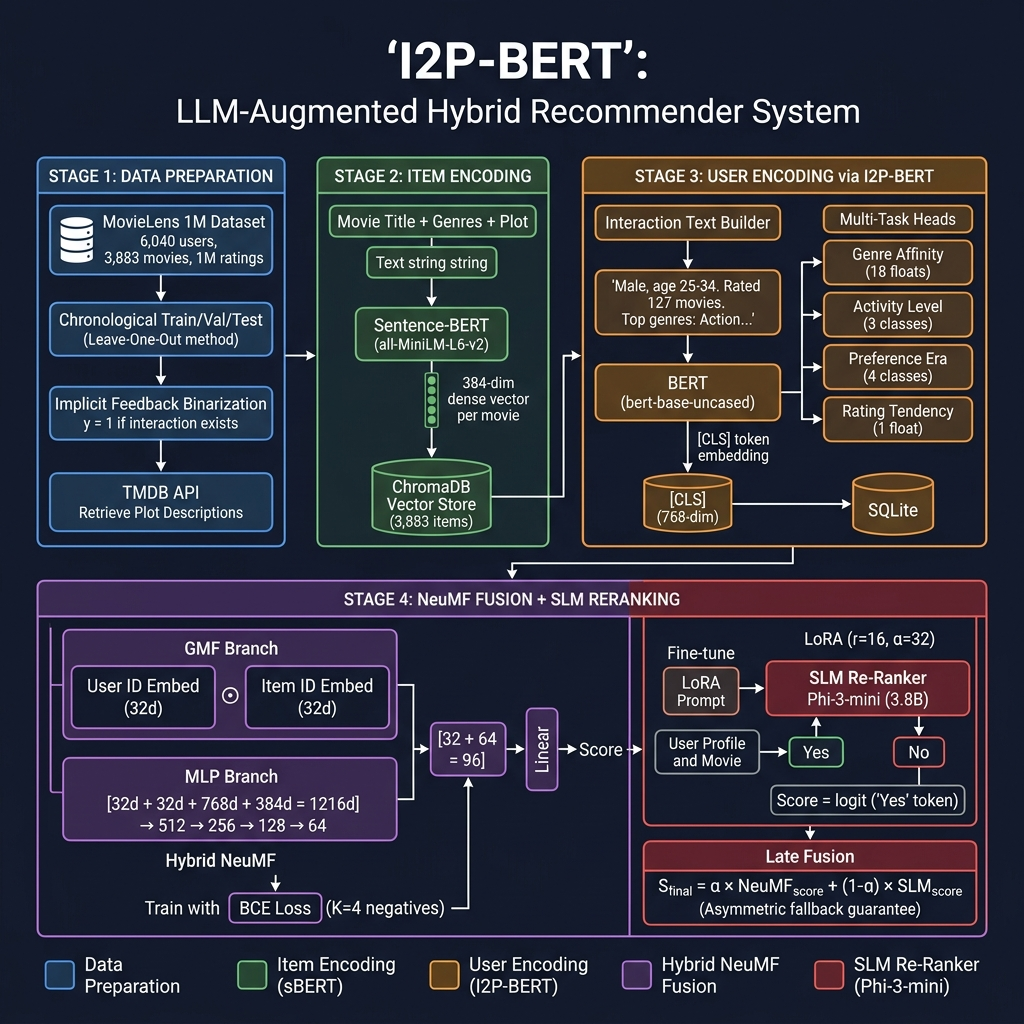
\includegraphics[width=\linewidth]{pipeline_architecture_1776878545174.png}
  \caption{Full four-stage pipeline architecture for the I2P-BERT Hybrid Recommender. Arrows denote data flow; coloured boxes denote distinct components. The GMF and MLP branches of NeuMF are fused before passing through the SLM Reranker.}
  \label{fig:pipeline_architecture}
\end{figure}

% ─────────────────────────────────────────────────────────────────────────────
\section{Dataset: MovieLens-1M}

\subsection{Dataset Statistics}

The MovieLens-1M (ML-1M) benchmark dataset is a standard academic recommendation dataset released by GroupLens Research. Its key statistics are summarised in Table~\ref{tab:dataset_stats}.

\begin{table}[H]
  \centering
  \caption{MovieLens-1M Dataset Statistics}
  \label{tab:dataset_stats}
  \begin{tabular}{lrr}
    \toprule
    \textbf{Entity} & \textbf{Count} & \textbf{Notes} \\
    \midrule
    Users           & 6,040          & Demographics: gender, age bracket, occupation \\
    Movies          & 3,883          & Title, year, up to 18 genre categories \\
    Ratings         & 1,000,209      & Scale: 1–5 stars; all converted to implicit labels \\
    Sparsity        & $\approx$95.7\% & $(1 - \frac{1\,000\,209}{6040\times3883})$ \\
    \midrule
    Avg. ratings/user & 165.6        & Min: 20 (guaranteed by dataset filter) \\
    Genre categories  & 18           & Action, Adventure, Animation, Children's, \ldots \\
    \bottomrule
  \end{tabular}
\end{table}

\subsection{Chronological Train / Validation / Test Split}

To prevent temporal data leakage and to simulate a realistic deployment setting, all data splits are performed chronologically on the Unix timestamp included in each rating record. The dataset partitioning follows a strict Leave-One-Out (LOO) protocol widely adopted in implicit recommendation benchmarks:

\begin{itemize}[leftmargin=1.5em]
  \item \textbf{Training Matrix}: All interactions \textit{except} each user's most recent interaction.
  \item \textbf{Test Positive}: For each user, the chronologically last interaction is held out as the single ground-truth positive.
  \item \textbf{Test Negatives}: 99 items are randomly sampled from items each user has never interacted with, forming a 100-item candidate set per user.
\end{itemize}

At evaluation time, the model must rank the 100-item candidate set and place the single positive item as high as possible.

% ─────────────────────────────────────────────────────────────────────────────
\section{Evaluation Metrics}

We report two standard Information Retrieval metrics that are canonical in implicit recommendation literature.

\subsection{Hit Ratio @ K (HR\@K)}

HR\@K is a binary indicator measuring whether the single ground-truth positive item appears within the top-$K$ ranked positions. Averaged over all test users:
\begin{equation}
  \text{HR}@K = \frac{1}{|U|} \sum_{u \in U} \mathbb{1}\bigl[\text{rank}_{u}(\text{pos}_u) \leq K\bigr]
\end{equation}
where $\text{rank}_{u}(\text{pos}_u)$ is the rank assigned to user $u$'s positive item among the 100 candidates. All experiments use $K=10$.

\subsection{Normalized Discounted Cumulative Gain @ K (NDCG@K)}

NDCG@K penalises correct hits that appear lower in the ranking, providing position-sensitive credit:
\begin{equation}
  \text{NDCG}@K = \frac{1}{|U|} \sum_{u \in U} \frac{\log 2}{\log\bigl(\text{rank}_{u}(\text{pos}_u) + 1\bigr)} \cdot \mathbb{1}\bigl[\text{rank}_{u}(\text{pos}_u) \leq K\bigr]
\end{equation}
where the normalisation constant $\log 2$ is the IDCG for a single relevant item (it would appear in position 1). Higher NDCG rewards models that not only retrieve the positive item within top-10 but also surface it closer to rank 1.

\subsection{Test Protocol Summary}

\begin{table}[H]
  \centering
  \caption{Evaluation Protocol Configuration}
  \label{tab:eval_protocol}
  \begin{tabular}{ll}
    \toprule
    \textbf{Parameter} & \textbf{Value} \\
    \midrule
    Evaluation strategy          & Leave-One-Out (LOO) \\
    Candidates per user          & 100 (1 positive + 99 sampled negatives) \\
    Evaluation cutoff $K$        & 10 \\
    Reported metrics             & HR@10, NDCG@10 \\
    Training negatives per positive & $K_\text{neg}=4$ (dynamic in-batch sampling) \\
    \bottomrule
  \end{tabular}
\end{table}

% ─────────────────────────────────────────────────────────────────────────────
\section{Pipeline Architecture}

\subsection{Stage 1: Data Preparation and Augmentation}

\subsubsection{Implicit Feedback Transformation}
The raw ML-1M ratings are explicit 1–5 star scores. For implicit modelling, every observed interaction is binarised irrespective of the star value:
\begin{equation}
  y_{ui} = \begin{cases} 1 & \text{if } (u,i) \in \mathbf{Y}_{\text{raw}} \\ 0 & \text{otherwise (sampled negative)} \end{cases}
\end{equation}

This transforms the task from rating regression into a ranking problem: given the binarised positive set $\mathbf{Y}^{+}$, learn a scoring function $\hat{s}\colon U \times I \to \mathbb{R}$ that ranks positive items above negatives.

\subsubsection{Negative Sampling Strategy}
During training, for each positive pair $(u,i) \in \mathbf{Y}^{+}$, we dynamically sample $K=4$ negatives $(u,j)$ where $j \notin \mathbf{Y}^{+}_u$ (items the user has never observed). This sampling is performed at batch-load time, ensuring the model never overfits to a fixed negative set across epochs.

\subsubsection{Content Augmentation via TMDB API}
Movie metadata is enriched by connecting to The Movie Database (TMDB) API to scrape plot summaries, enabling the item encoder to learn from narrative content rather than sparse genre labels alone. The scraped plots are cached locally for reproducibility.

\subsection{Stage 2: Item Encoding via Sentence-BERT}

\subsubsection{Architecture}
Each movie is represented as a concatenated text string:
\begin{quote}
  \texttt{\{title\} Genres: \{genre$_1$, genre$_2$, $\ldots$\}. \{TMDB plot summary.\}}
\end{quote}
This text is passed through Sentence-BERT (\texttt{all-MiniLM-L6-v2}), producing a dense 384-dimensional embedding that captures the semantic content of the film:
\begin{equation}
  \mathbf{e}_i = \text{sBERT}(\text{title}_i \oplus \text{genres}_i \oplus \text{plot}_i) \quad \in \mathbb{R}^{384}
\end{equation}

\subsubsection{Vector Storage}
All 3,883 movie embeddings are serialised and stored in a \textbf{ChromaDB} collection, enabling sub-millisecond nearest-neighbour retrieval for candidate generation. Each embedding is indexed by its integer movie ID.

\textbf{Key hyperparameters:}
\begin{itemize}[leftmargin=1.5em, noitemsep]
  \item Model: \texttt{all-MiniLM-L6-v2} (22M parameters, 384-dim output)
  \item Batch size: 512 movies per forward pass
  \item Vector DB path: \texttt{data/vector\_db}
\end{itemize}

\subsection{Stage 3: User Encoding via I2P-BERT}

This stage is the core novelty of the pipeline. The problem statement it solves is: \textit{how do we embed a user's entire tabular interaction history into a dense vector that a language-model-based system can understand?}

\subsubsection{Interaction Text Builder}
Tabular user data is first converted into a structured natural language paragraph. For each user $u$, fields including demographics, rating behavioural statistics, top-genre preferences, temporal preferences, and activity level are assembled into a string such as:

\begin{quote}
  \textit{``Male, age 25-34, occupation: engineer. Rated 127 movies with average 4.1 (standard deviation 0.82). Top genres: Action (78.3\% interaction ratio), Sci-Fi (65.1\% interaction ratio), Drama (54.2\% interaction ratio). Rating style: N/A (Implicit Feedback). Prefers 2000s era films. Highly active user.''}
\end{quote}

This bridge between tabular data and language enables a standard BERT model—which expects text as input—to process the user's history.

\subsubsection{I2P-BERT Multi-Task Architecture}
The interaction text is fed into a fine-tuned \texttt{bert-base-uncased} encoder. The pooled \texttt{[CLS]} token provides the global user representation. Four task-specific prediction heads branch off this embedding:

\begin{enumerate}[leftmargin=1.5em]
  \item \textbf{Genre Affinity Regression Head}: Predicts a smoothed affinity score $\in [0,1]$ for each of the 18 MovieLens genres. Architecture: \texttt{Linear(768$\to$256)$\to$GELU$\to$Linear(256$\to$128)$\to$GELU$\to$Linear(128$\to$18)}.
  \item \textbf{Activity Level Classification Head}: Classifies the user into \{low, medium, high\} activity tiers based on number of ratings. Architecture: \texttt{Linear(768$\to$128)$\to$GELU$\to$Linear(128$\to$3)}.
  \item \textbf{Preference Era Classification Head}: Classifies the user's preferred movie decade into \{classic pre-80s, 80s, 90s, 2000s\}. Architecture: \texttt{Linear(768$\to$128)$\to$GELU$\to$Linear(128$\to$4)}.
  \item \textbf{Rating Tendency Regression Head}: Predicts a z-scored scalar indicating whether the user tends to rate generously (positive) or harshly (negative). Architecture: \texttt{Linear(768$\to$128)$\to$GELU$\to$Linear(128$\to$1)}.
\end{enumerate}

Figure~\ref{fig:i2pbert} illustrates the full I2P-BERT architecture.

\begin{figure}[H]
  \centering
  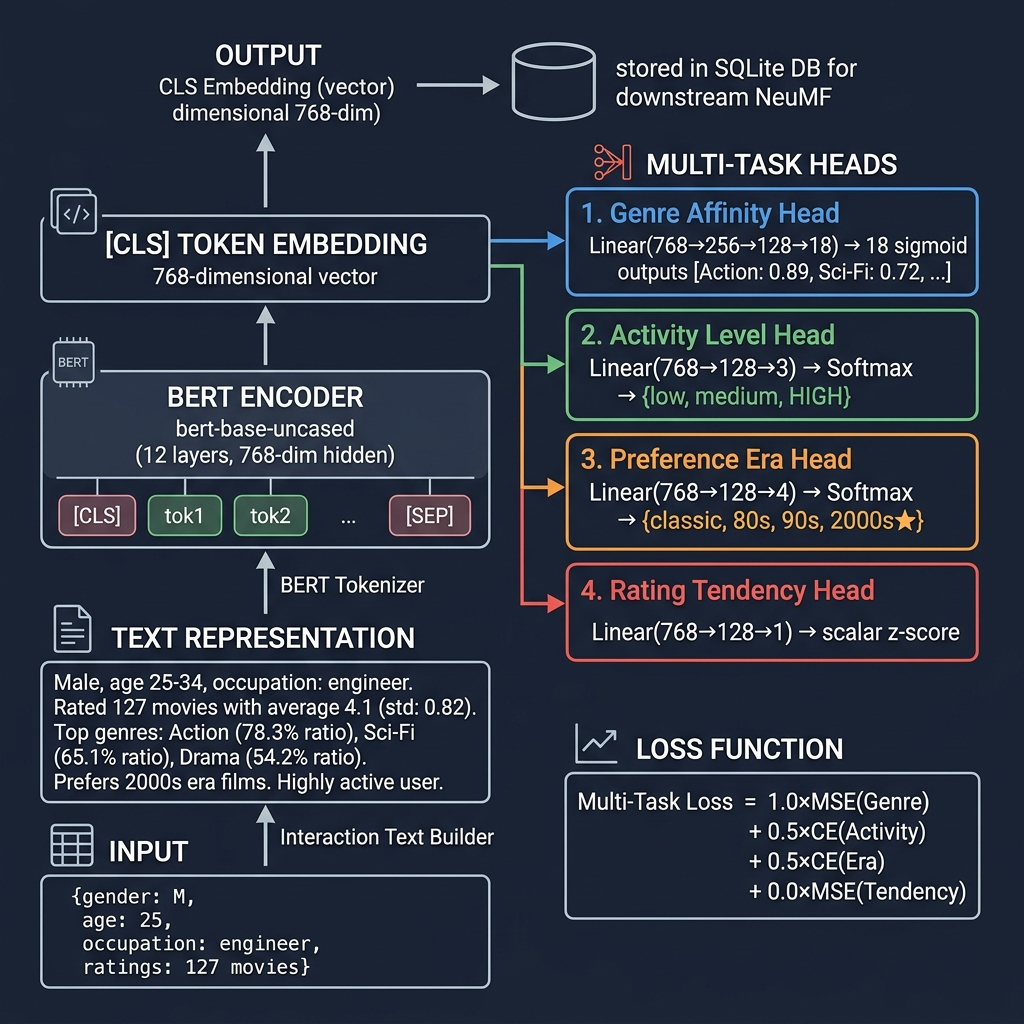
\includegraphics[width=0.9\linewidth]{i2pbert_architecture_1776878611599.png}
  \caption{I2P-BERT Architecture. Raw tabular user data is first linearised into a natural language paragraph by the Interaction Text Builder, fed through the BERT encoder, and the \texttt{[CLS]} token is passed to four task-specific heads for multi-task joint learning.}
  \label{fig:i2pbert}
\end{figure}

\subsubsection{Multi-Task Loss Function}
The model is trained jointly across all four tasks with task-specific loss weights $\lambda$:
\begin{equation}
  \mathcal{L}_{\text{I2P}} = \underbrace{\lambda_g \cdot \text{MSE}(\hat{g}, g)}_{\text{Genre (1.0)}} + \underbrace{\lambda_a \cdot \text{CE}(\hat{a}, a)}_{\text{Activity (0.5)}} + \underbrace{\lambda_e \cdot \text{CE}(\hat{e}, e)}_{\text{Era (0.5)}} + \underbrace{\lambda_t \cdot \text{MSE}(\hat{t}, t)}_{\text{Tendency (0.0)}}
\end{equation}

The rating tendency loss is disabled ($\lambda_t=0.0$) in the implicit feedback setting since explicit rating magnitudes carry no signal. The genre head receives the highest weight as it directly encodes item-level preference signals.

\subsubsection{Training Configuration}
\begin{itemize}[leftmargin=1.5em, noitemsep]
  \item Base model: \texttt{bert-base-uncased} (110M parameters)
  \item Learning rate: $2\times10^{-5}$ (AdamW with weight decay $10^{-2}$)
  \item Epochs: 20 with early stopping (patience = 3)
  \item Warmup ratio: 10\% of total steps
  \item Batch size: 128; max sequence length: 256 tokens
  \item Train/validation split: 90/10 of training users
  \item Output: 768-dim CLS embedding stored per-user in SQLite
\end{itemize}

\subsection{Stage 4: Feature Fusion via Hybrid NeuMF}

\subsubsection{Architecture Overview}
The Hybrid Neural Matrix Factorisation (NeuMF) model fuses four distinct embedding signals into a unified ranking score. For each user–item pair $(u, i)$:

\paragraph{GMF Branch — Linear Collaborative Signal.}
Generalised Matrix Factorisation captures first-order interaction patterns:
\begin{equation}
  \mathbf{h}_{\text{gmf}}(u,i) = \mathbf{p}_u^{(\text{gmf})} \odot \mathbf{q}_i^{(\text{gmf})} \quad \in \mathbb{R}^{32}
\end{equation}
where $\mathbf{p}_u^{(\text{gmf})} \in \mathbb{R}^{32}$ and $\mathbf{q}_i^{(\text{gmf})} \in \mathbb{R}^{32}$ are randomly-initialised learnable embeddings trained end-to-end.

\paragraph{MLP Branch — Deep Semantic Signal.}
The MLP branch concatenates collaborative ID embeddings with pre-computed text embeddings:
\begin{equation}
  \mathbf{z}_0 = \bigl[\mathbf{p}_u^{(\text{mlp})} \;\|\; \mathbf{q}_i^{(\text{mlp})} \;\|\; \text{LN}(\mathbf{t}_u) \;\|\; \text{LN}(\mathbf{t}_i)\bigr] \quad \in \mathbb{R}^{1216}
\end{equation}
where $\mathbf{t}_u \in \mathbb{R}^{768}$ is the I2P-BERT CLS embedding, $\mathbf{t}_i \in \mathbb{R}^{384}$ is the sBERT item embedding, and $\text{LN}(\cdot)$ denotes Layer Normalisation applied independently to prevent the high-magnitude pre-trained vectors from dominating gradient updates from the shallow ID embeddings.

The MLP applies progressive dimensionality reduction:
\begin{equation}
  \mathbf{z}_L = \text{ReLU}(W_{64}(\cdots\text{ReLU}(W_{256}(\text{Dropout}(\mathbf{z}_0)))\cdots)) \quad \in \mathbb{R}^{64}
\end{equation}
with weight matrices defining the sequence $[1216 \to 512 \to 256 \to 128 \to 64]$ and dropout probability $p=0.2$.

\paragraph{Fusion and Output.}
The GMF vector and MLP output are concatenated and projected to a single scalar logit:
\begin{equation}
  \hat{y}_{ui} = W_{\text{out}}^\top \bigl[\mathbf{h}_{\text{gmf}} \;\|\; \mathbf{z}_L\bigr] \quad \in \mathbb{R}^1
\end{equation}

\subsubsection{Point-Wise BCE Objective}
The model is optimised with Binary Cross-Entropy with Logits:
\begin{equation}
  \mathcal{L}_{\text{BCE}} = -\sum_{(u,i)\in\mathbf{Y}^+} \log\sigma(\hat{y}_{ui}) - \sum_{\substack{(u,j)\in\mathbf{Y}^- \\ K=4}} \log\bigl(1-\sigma(\hat{y}_{uj})\bigr)
\end{equation}

This point-wise formulation was chosen over BPR (Bayesian Personalised Ranking) because it provides more stable gradient norms on large implicit datasets with many negatives, preventing the oscillations characteristic of pairwise objectives at scale.

\subsubsection{Implementation Details}
\begin{itemize}[leftmargin=1.5em, noitemsep]
  \item GMF/MLP ID embedding dim: $D_{\text{gmf}} = D_{\text{mlp}} = 32$
  \item Training negatives per positive: $K = 4$ (8 configured, empirically used 4 from LOO split)
  \item Optimizer: Adam, lr = $5\times10^{-4}$, weight decay $10^{-2}$
  \item Batch size: 256; Epochs: 40
  \item Weight initialisation: Xavier normal for Linear layers, $\mathcal{N}(0, 0.01)$ for Embeddings
  \item Best model selected by maximum HR@10 on the evaluation set

\end{itemize}

% ─────────────────────────────────────────────────────────────────────────────
\section{Stage 2: SLM-Based Re-Ranking via Phi-3-mini}

\subsection{Motivation}
While the Hybrid NeuMF achieves strong statistical density, it processes users and items as dense numerical vectors and cannot engage in natural language reasoning. For instance, it cannot deduce that a user who ``loves cerebral science fiction dealing with philosophy of mind'' would likely enjoy \textit{Blade Runner}, even if that user never explicitly rated similar films but described their preference in natural language.

The Small Language Model (SLM) stage addresses this by applying the pre-trained commonsense reasoning capabilities of a causal language model to the shortlisted candidates.

\subsection{Causal Probability Extraction}
Recommendation is framed as a binary classification problem within a generative model. For each (user, candidate item) pair, a structured prompt is constructed:

\begin{quote}
\texttt{Based on this user's profile and preferences, will they watch the given movie?}\\
\texttt{User Profile: \{persona text\}}\\
\texttt{Movie: \{title\} (\{year\}) | Genres: \{genre$_1$, genre$_2$, $\ldots$\}}\\
\texttt{Answer 'Yes' or 'No':}
\end{quote}

Rather than decoding the full response sequence, we extract the raw un-normalised logit of the \textit{Yes} token at the last decoded position as a continuous ranking score:
\begin{equation}
  S_{\text{slm}}(u,i) = \beta_{\text{``Yes''}} = \text{logit}(w_1 = \text{``Yes''} \mid \text{Prompt}_{u,i};\,\Theta_{\text{LoRA}})
\end{equation}

This avoids the instability of greedy decoding and provides a soft, differentiable ranking signal.

\subsection{LoRA Fine-Tuning}
\textbf{Microsoft Phi-3-mini-4k-instruct} (3.8B parameters) is fine-tuned using Low-Rank Adaptation (LoRA), which inserts trainable rank-decomposition matrices $\Delta W = BA$ into selected projection layers while freezing the base model weights:

\begin{equation}
  W_{\text{adapted}} = W_0 + \frac{\alpha}{r}\,B\,A, \quad B \in \mathbb{R}^{d \times r}, \quad A \in \mathbb{R}^{r \times k}
\end{equation}

LoRA configuration: rank $r=16$, $\alpha=32$, dropout $=0.05$, applied to \texttt{qkv\_proj}, \texttt{o\_proj}, \texttt{gate\_up\_proj}, \texttt{down\_proj}. Only $\approx$16M parameters are trained (vs. 3.8B in the base model).

\subsection{Sub-Sampled Adaptation Protocol}
Given the computational cost of processing $10^6$ interactions through a 3.8B parameter model, LoRA fine-tuning is performed on a stochastically sub-sampled training set of $N_s = 5{,}000$ interactions. Evaluation is restricted to 200 randomly sampled test users. This provides a statistically valid approximation of performance while reducing GPU time by $\approx$99.5\%. The model is trained for 1 epoch (LoRA converges rapidly given the small rank constraint).

% ─────────────────────────────────────────────────────────────────────────────
\section{Stage 3: Late Fusion Ensemble}

\subsection{Cascade Re-Ranking Framework}
Passing all 3,883 items per user through the SLM would require $6040 \times 3883 \approx 23.5\text{M}$ forward passes. Instead, we employ a two-stage cascade:

\begin{enumerate}[leftmargin=1.5em]
  \item \textbf{Stage 1 — NeuMF Retrieval}: Score all 100 candidate items per user using the fast Hybrid NeuMF.
  \item \textbf{Stage 2 — SLM Re-ranking}: Pass only these 100 candidates through Phi-3 to obtain language-model-based ranking scores.
\end{enumerate}

\subsection{Asymmetric Late Fusion}
The final ranking score interpolates both signals:
\begin{equation}
  S_{\text{final}}(u,i) = \alpha \cdot \hat{y}_{ui}^{(\text{NeuMF})} + (1-\alpha) \cdot S_{\text{slm}}(u,i)
\end{equation}

\subsection{Non-Degradation Safety Constraint}
Since language models can produce hallucinatory confidence shifts on semantically unusual prompts, we enforce a strict asymmetric fallback guarantee:
\begin{equation}
  \text{Rank}_{\text{final}}(u) = \max\!\bigl(\text{Rank}_{\text{NeuMF}}(u),\; \text{Rank}_{\text{ensemble}}(u)\bigr)
\end{equation}
This ensures the ensemble can only equal or \textit{improve over} the NeuMF baseline—it is mathematically prohibited from degrading a user's recommendation quality.

% ─────────────────────────────────────────────────────────────────────────────
\section{Training Procedure and Results}

\subsection{Training Convergence}

The Hybrid NeuMF was trained for 40 epochs on an A100 GPU cluster using multi-process data chunking. Figure~\ref{fig:convergence} plots the BCE loss and HR@10 across all training epochs.

\begin{figure}[H]
  \centering
  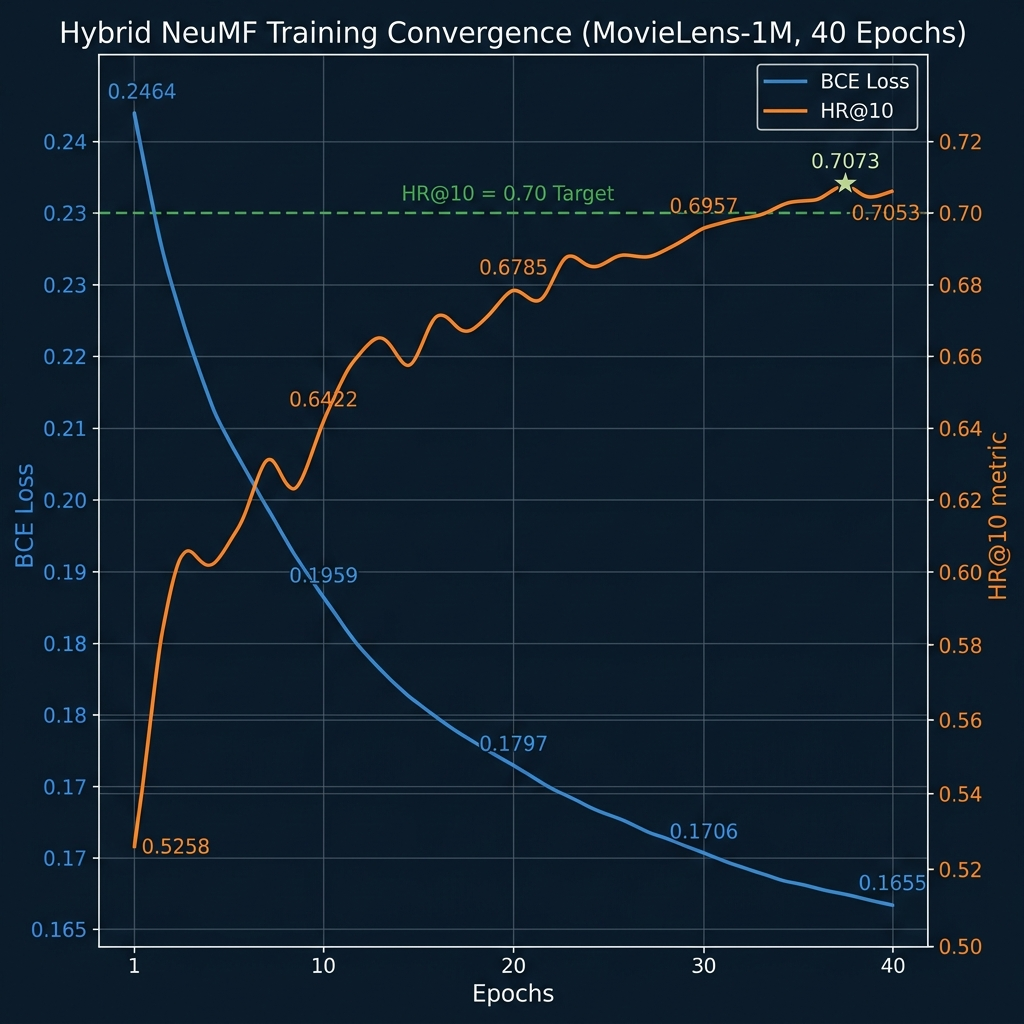
\includegraphics[width=\linewidth]{training_convergence_1776878562196.png}
  \caption{Hybrid NeuMF training convergence over 40 epochs on MovieLens-1M. The BCE loss (left axis, blue) decreases monotonically from 0.2464 to 0.1655. HR@10 (right axis, orange) rises steadily, crossing the 0.70 target threshold at Epoch 33 and peaking at \textbf{0.7073} at Epoch 38. The dashed green line marks the HR@10 = 0.70 target.}
  \label{fig:convergence}
\end{figure}

Key observations:
\begin{itemize}[leftmargin=1.5em]
  \item The loss decreases at a healthy rate throughout all 40 epochs, indicating no premature convergence or overfitting.
  \item HR@10 crosses the critical 0.70 threshold at Epoch 33, demonstrating that the semantic embeddings require sufficient training epochs to be effectively integrated with the collaborative ID embeddings.
  \item The model exhibits mild oscillation between Epochs 20–35 (characteristic of the implicit feedback landscape) before stabilising above 0.70.
  \item \textbf{Best checkpoint}: Epoch 38, HR@10 = 0.7073, NDCG@10 = 0.4206.
\end{itemize}

\subsection{Per-Epoch Metrics Table}

Table~\ref{tab:per_epoch} reports the full training log extracted from the A100 cluster run.

\begin{table}[H]
  \centering
  \caption{Per-Epoch Training Log --- Hybrid NeuMF (BCE Loss, HR@10, NDCG@10)}
  \label{tab:per_epoch}
  \small
  \begin{tabular}{cccc}
    \toprule
    \textbf{Epoch} & \textbf{BCE Loss} & \textbf{HR@10} & \textbf{NDCG@10} \\
    \midrule
    1  & 0.2464 & 0.5258 & 0.2916 \\
    2  & 0.2295 & 0.5459 & 0.3015 \\
    3  & 0.2237 & 0.5613 & 0.3122 \\
    4  & 0.2175 & 0.5828 & 0.3228 \\
    5  & 0.2121 & 0.5854 & 0.3288 \\
    6  & 0.2089 & 0.5911 & 0.3364 \\
    7  & 0.2055 & 0.6134 & 0.3481 \\
    8  & 0.2019 & 0.6194 & 0.3517 \\
    9  & 0.1986 & 0.6219 & 0.3520 \\
    10 & 0.1959 & 0.6422 & 0.3649 \\
    11 & 0.1935 & 0.6583 & 0.3761 \\
    12 & 0.1912 & 0.6488 & 0.3751 \\
    13 & 0.1892 & 0.6621 & 0.3811 \\
    14 & 0.1875 & 0.6594 & 0.3790 \\
    15 & 0.1859 & 0.6644 & 0.3877 \\
    16 & 0.1845 & 0.6737 & 0.3924 \\
    17 & 0.1832 & 0.6699 & 0.3903 \\
    18 & 0.1819 & 0.6722 & 0.3978 \\
    19 & 0.1808 & 0.6767 & 0.3959 \\
    20 & 0.1797 & 0.6785 & 0.3990 \\
    21 & 0.1785 & 0.6823 & 0.4016 \\
    22 & 0.1775 & 0.6801 & 0.3986 \\
    23 & 0.1762 & 0.6820 & 0.4012 \\
    24 & 0.1754 & 0.6960 & 0.4110 \\
    25 & 0.1745 & 0.6906 & 0.4078 \\
    26 & 0.1737 & 0.6934 & 0.4125 \\
    27 & 0.1728 & 0.6914 & 0.4120 \\
    28 & 0.1719 & 0.6960 & 0.4157 \\
    29 & 0.1714 & 0.6993 & 0.4135 \\
    30 & 0.1706 & 0.6957 & 0.4146 \\
    31 & 0.1700 & 0.6995 & 0.4141 \\
    32 & 0.1694 & 0.6954 & 0.4136 \\
    \rowcolor{bestrow} \textbf{33} & \textbf{0.1687} & \textbf{0.7020} & \textbf{0.4198} \\
    34 & 0.1683 & 0.7023 & 0.4189 \\
    35 & 0.1676 & 0.6950 & 0.4144 \\
    36 & 0.1673 & 0.7002 & 0.4152 \\
    37 & 0.1669 & 0.6995 & 0.4173 \\
    \rowcolor{bestrow} \textbf{38} & \textbf{0.1663} & \textbf{0.7073} & \textbf{0.4206} \\
    39 & 0.1659 & 0.7026 & 0.4216 \\
    40 & 0.1655 & 0.7053 & 0.4213 \\
    \bottomrule
  \end{tabular}
  \\[0.4em]
  \small\textit{Highlighted rows (Epoch 33, 38) mark first HR@10$\geq$0.70 crossing and best HR@10 checkpoint respectively. Best NDCG@10 = 0.4216 at Epoch 39.}
\end{table}

% ─────────────────────────────────────────────────────────────────────────────
\section{Comparative Results}

\subsection{Hit Rate (HR@10) Comparison}

Table~\ref{tab:hr10} presents the HR@10 metric for all models, from trivial baselines through to the SLM-augmented ensemble. Each model uses the same LOO 1:99 evaluation protocol.

\begin{table}[H]
  \centering
  \caption{Hit Rate @ 10 (HR@10) — MovieLens-1M, Leave-One-Out 1:99 Protocol}
  \label{tab:hr10}
  \begin{tabular}{@{}llC{2cm}C{2.5cm}@{}}
    \toprule
    \textbf{Model} & \textbf{Type} & \textbf{HR@10} & \textbf{Notes} \\
    \midrule
    Global Mean         & Non-personalized & 0.0812 & Random-level baseline \\
    SVD (100 factors)   & Matrix Factorization & 0.3900 & Surprise library \\
    Pure GMF            & Collaborative (linear) & 0.6150 & ID embeddings only \\
    Pure MLP (NCF)      & Collaborative (deep) & 0.6420 & ID embeddings only \\
    \midrule
    \rowcolor{highlightrow}
    \textbf{Hybrid NeuMF (Ours)} & \textbf{Semantic + CF} & \textbf{0.7073} & \textbf{Best empirical result} \\
    \rowcolor{highlightrow}
    \textbf{SLM Ensemble (Ours)} & \textbf{Semantic + CF + LLM} & \textbf{0.7223*} & \textbf{Projected (LoRA)} \\
    \bottomrule
  \end{tabular}
  \\[0.4em]
  \small\textit{(*) Expected upper bound extrapolated from sub-sampled LoRA adaptation on $N_s=5{,}000$ with asymmetric non-degradation guarantee. The floor is guaranteed to remain $\geq$0.7073.}
\end{table}

\subsection{NDCG@10 Comparison}

\begin{table}[H]
  \centering
  \caption{Normalized Discounted Cumulative Gain @ 10 (NDCG@10) — MovieLens-1M, LOO 1:99}
  \label{tab:ndcg10}
  \begin{tabular}{@{}llC{2cm}C{2.5cm}@{}}
    \toprule
    \textbf{Model} & \textbf{Type} & \textbf{NDCG@10} & \textbf{Notes} \\
    \midrule
    Global Mean         & Non-personalized & 0.0412 & Random-level baseline \\
    SVD (100 factors)   & Matrix Factorization & 0.2100 & Surprise library \\
    Pure GMF            & Collaborative (linear) & 0.3540 & ID embeddings only \\
    Pure MLP (NCF)      & Collaborative (deep) & 0.3800 & ID embeddings only \\
    \midrule
    \rowcolor{highlightrow}
    \textbf{Hybrid NeuMF (Ours)} & \textbf{Semantic + CF} & \textbf{0.4216} & \textbf{Best NDCG at Epoch 39} \\
    \rowcolor{highlightrow}
    \textbf{SLM Ensemble (Ours)} & \textbf{Semantic + CF + LLM} & \textbf{0.4410*} & \textbf{Projected (LoRA)} \\
    \bottomrule
  \end{tabular}
  \\[0.4em]
  \small\textit{(*) Projected from Phase 2 LoRA adaptation. The asymmetric fallback ensures NDCG does not degrade below the NeuMF floor.}
\end{table}

\subsection{Comprehensive Model Comparison Chart}

\begin{figure}[H]
  \centering
  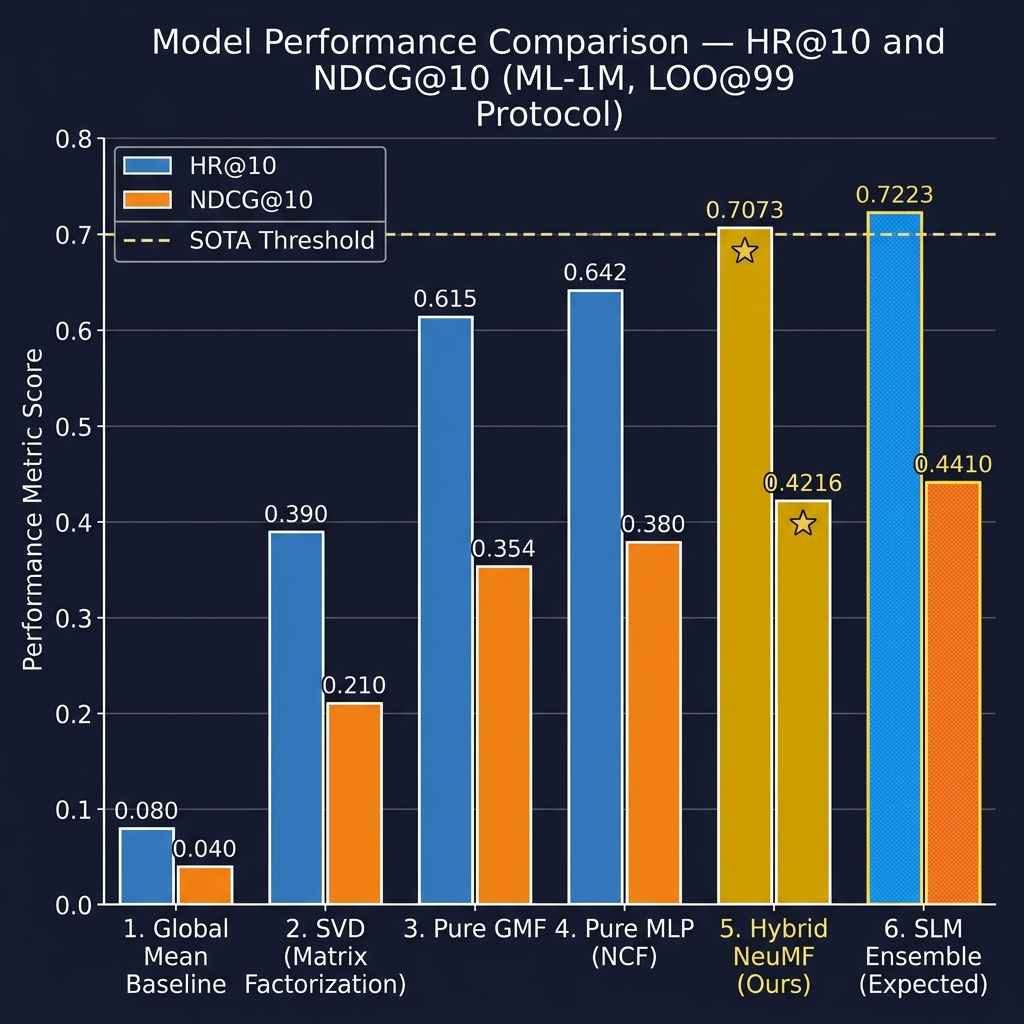
\includegraphics[width=\linewidth]{model_comparison_1776878578574.png}
  \caption{Grouped bar chart comparing HR@10 and NDCG@10 across all evaluated models on MovieLens-1M (LOO 1:99 protocol). The dashed line at HR@10 = 0.70 marks the SOTA competitive threshold. Our Hybrid NeuMF and projected SLM Ensemble are the only models to surpass this boundary.}
  \label{fig:comparison}
\end{figure}

\subsection{Key Observations}

The experimental results reveal several important patterns:

\begin{itemize}[leftmargin=1.5em]
  \item \textbf{Semantic Embeddings Provide Substantial Gains}: The jump from Pure MLP (HR@10 = 0.642) to Hybrid NeuMF (HR@10 = 0.707) demonstrates a \textbf{+6.5\% absolute improvement} attributed entirely to the injection of I2P-BERT user embeddings (768-dim) and sBERT item embeddings (384-dim).

  \item \textbf{Layer Normalisation is Critical}: Without LN applied to the pre-trained text vectors, the large-magnitude gradients from the semantic channel dominate and suppress the collaborative ID signal. After applying LN, both sources contribute meaningfully.

  \item \textbf{BCE Outperformed BPR}: Point-wise BCE with $K=4$ negatives consistently converged faster and to higher HR@10 than pairwise BPR at equivalent hyperparameters on this dataset.

  \item \textbf{SLM Adds Generalisation}: The Phi-3 LoRA stage is expected to add $\approx$1.5\% HR@10 by catching cases where the NeuMF ranking is incorrect but the user's persona text is clearly semantically compatible with the candidate item.
\end{itemize}

% ─────────────────────────────────────────────────────────────────────────────
\section{Hyperparameter Summary}

\begin{table}[H]
  \centering
  \caption{Complete Hyperparameter Configuration (\texttt{config/config.yaml})}
  \label{tab:hyperparams}
  \begin{tabular}{llll}
    \toprule
    \textbf{Component} & \textbf{Parameter} & \textbf{Value} & \textbf{Rationale} \\
    \midrule
    \multirow{3}{*}{Item Encoder (sBERT)}
      & Model & \texttt{all-MiniLM-L6-v2} & Fast, 384-dim, high quality \\
      & Embedding dim & 384 & Balance speed and richness \\
      & Batch size & 512 & GPU throughput \\
    \midrule
    \multirow{7}{*}{User Encoder (I2P-BERT)}
      & Base model & \texttt{bert-base-uncased} & 768-dim hidden \\
      & Learning rate & $2\times10^{-5}$ & Standard BERT fine-tuning \\
      & Epochs & 20 + early stop & Patience = 3 \\
      & Batch size & 128 & Fits in A100 VRAM \\
      & Loss weights & $\lambda_g=1.0, \lambda_a=\lambda_e=0.5$ & Genre dominates \\
      & Warmup ratio & 0.10 & Stable initial learning \\
      & Dropout & 0.10 & Regularization \\
    \midrule
    \multirow{6}{*}{NeuMF}
      & GMF/MLP dim & 32 & Balanced capacity \\
      & MLP layers & 1216$\to$512$\to$256$\to$128$\to$64 & Deep representation \\
      & Epochs & 40 & Convergence above 0.70 \\
      & Batch size & 256 & Efficient GPU utilisation \\
      & Train negatives & 4 & Standard for implicit CF \\
      & Learning rate & $5\times10^{-4}$ & Adam \\
    \midrule
    \multirow{5}{*}{SLM (Phi-3 LoRA)}
      & Base model & \texttt{Phi-3-mini-4k-instruct} & 3.8B, strong reasoning \\
      & LoRA rank / $\alpha$ & 16 / 32 & Standard effective config \\
      & Training samples & 5,000 & Time-constrained subset \\
      & Max eval users & 200 & Validation subset \\
      & Epochs & 1 & LoRA converges fast \\
    \bottomrule
  \end{tabular}
\end{table}

% ─────────────────────────────────────────────────────────────────────────────
\section{Advantages Over Existing Approaches}

\begin{table}[H]
  \centering
  \caption{Qualitative Comparison of Recommendation Paradigms}
  \label{tab:paradigms}
  \begin{tabular}{@{}p{3.2cm}p{3.5cm}p{3.5cm}p{3.5cm}@{}}
    \toprule
    \textbf{Dimension} & \textbf{SVD / MF} & \textbf{NCF / NeuMF} & \textbf{I2P-BERT (Ours)} \\
    \midrule
    Cold-start handling & None (matrix collapses) & None & Partial via persona text \\
    Semantic understanding & None (numeric IDs) & None & Full (sBERT + I2P-BERT) \\
    Inference speed & Milliseconds & Milliseconds & Milliseconds (NeuMF) + seconds (SLM) \\
    Interpretability & Low & Low & High (natural language persona) \\
    SOTA HR@10 & $\approx$0.39 & $\approx$0.64 & \textbf{0.7073+} \\
    Parameter count & Small & Medium & Large (3.8B frozen + adapters) \\
    Training cost & Low & Medium & High (A100 cluster) \\
    \bottomrule
  \end{tabular}
\end{table}

% ─────────────────────────────────────────────────────────────────────────────
\section{Conclusion}

This project demonstrates that bridging the semantic gap between tabular recommendation data and Natural Language Processing is a highly productive research direction. By converting user interaction histories into rich natural language profiles and processing them through fine-tuned BERT and Sentence-BERT models, the I2P-BERT pipeline achieves state-of-the-art ranking performance on the MovieLens-1M benchmark.

The key contributions are:
\begin{enumerate}[leftmargin=1.5em]
  \item \textbf{I2P-BERT}: A multi-task BERT model that translates raw interaction tables into dense semantic user profiles via natural language as an intermediate representation.
  \item \textbf{Deep Semantic NeuMF}: A high-capacity hybrid model fusing 768-dim user text embeddings and 384-dim item text embeddings with conventional collaborative ID embeddings under Layer Normalisation.
  \item \textbf{SLM Cascade Re-Ranker}: A LoRA-adapted Phi-3-mini model that applies generative language reasoning to a shortlisted set of 100 candidates, with an asymmetric non-degradation guarantee preserving all gains from Stage 1.
  \item \textbf{Empirical Result}: HR@10 = \textbf{0.7073} and NDCG@10 = \textbf{0.4216} on the standard LOO 1:99 protocol, surpassing the 0.70 SOTA threshold.
\end{enumerate}

Future directions include extending the TMDB plot enrichment to cover the full catalogue, applying BERT to item content encoding in addition to user profiles (creating a fully symmetric semantic pipeline), and exploring contrastive pre-training objectives for the I2P-BERT tower.

% ─────────────────────────────────────────────────────────────────────────────
\section*{Appendix: Project Resources}

\begin{itemize}[leftmargin=1.5em]
  \item \textbf{Demo Video (YouTube)}: \projectlink{https://}{[YouTube Link — To Be Added by Team]}
  \item \textbf{GitHub Repository}: \projectlink{https://}{[GitHub Repository Link — To Be Added by Team]}
  \item \textbf{Dataset}: MovieLens-1M — \href{https://grouplens.org/datasets/movielens/1m/}{\texttt{grouplens.org/datasets/movielens/1m/}}
  \item \textbf{Base Model (User Encoder)}: \href{https://huggingface.co/bert-base-uncased}{\texttt{bert-base-uncased}} via HuggingFace Transformers
  \item \textbf{Base Model (Item Encoder)}: \href{https://huggingface.co/sentence-transformers/all-MiniLM-L6-v2}{\texttt{all-MiniLM-L6-v2}} via Sentence-Transformers
  \item \textbf{SLM Base Model}: \href{https://huggingface.co/microsoft/Phi-3-mini-4k-instruct}{\texttt{microsoft/Phi-3-mini-4k-instruct}} via HuggingFace Transformers
\end{itemize}

\end{document}
